\section{Results}

The code was tested using a video with 601 frames, each made by 1280x720 pixels. The results are obtained through a bash script, that runs the two parallel implementations for several values of the \emph{nw} parameter; for each configuration, the script performs ten runs, in order to have more reliable values.

In Figure \ref{fig:speedup} there are the curves for the speedup metrics. It is also included a curve for the ideal speedup, which is $f(n) = n$. As expected, we have an initial increase when the number of workers is low, and in particular smaller than 32, which is the number of cores of the machine; in this situation, the standard thread implementation quite follows the ideal curve, while the FastFlow implementation is a little bit lower. When the number of cores increases, becoming greater than 32, we have a drop in performances, and the speedup remains more or less stable.

In Figure \ref{fig:efficiency} we have instead the curves for the efficiency metrics; also in this case, there is the curve for the ideal efficiency, which is $f(n)=1$. These curves follows more or less the behavior of the speedup: at first, with small \emph{nw}, the efficiency is close to 1; then it drops and it starts to assume very small values.

The drops in performance are expected because, when the number of threads approaches the number of real cores of the machine, the system spends more time to orchestrate the computation among the workers, therefore increasing the completion time. This situation gets even worse when \emph{nw} is greater than the number of real cores, when we see a huge drop in efficiency, because of the overheads induced by threads management.

\begin{figure}[h]
    \begin{subfigure}{.49\textwidth}
    \centering
    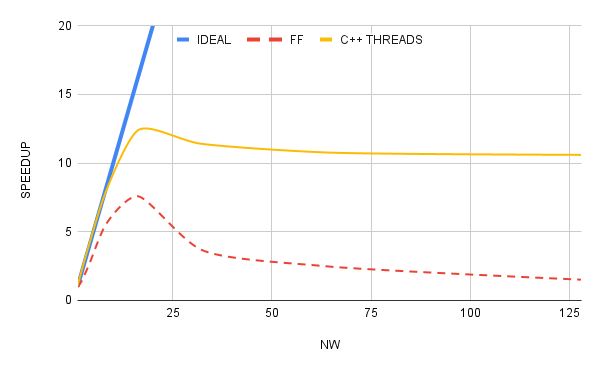
\includegraphics[width=\textwidth]{img/speed_up.png}
    \caption{Speedup}
    \label{fig:speedup}
    \end{subfigure}
    \begin{subfigure}{.49\textwidth}
    \centering
    \captionsetup{justification=centering}
    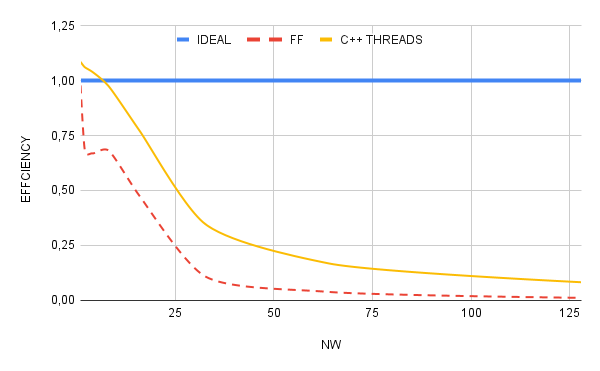
\includegraphics[width=\textwidth]{img/efficiency.png}
    \caption{Efficiency}
    \label{fig:efficiency}
    \end{subfigure} 
    \caption{}
    \label{fig:metrics}
\end{figure}

\section{Conclusion}
We saw a comparison between the sequential code and two parallel implementations performing the video motion detection.
The parallel implementations, especially with the right number of workers, offer a noticeable improvement with respect to the sequential implementation. I think that the speedup may be bigger if the computation was heavier, and in this context that may occur using a bigger matrix for the convolution in the smoothing process.\\
The development of this project gave me the opportunity to appreciate the difference between a standard C++ thread implementation and one using an high-level framework like FastFlow, which hides all the complexity and makes the implementation much easier and faster. The fact that the FastFlow implementation was a little bit less faster than the other one is maybe due to some error or missing optimization in the code.